% IEEE Conference Paper
% Compile with: pdflatex freshway_ieee_paper_corrected.tex
% Requires: IEEEtran class (standard in most LaTeX distributions)

\documentclass[conference]{IEEEtran}
\IEEEoverridecommandlockouts

% ─── PACKAGES ────────────────────────────────────────────────────────────────
\usepackage{cite}
\usepackage{amsmath,amssymb,amsfonts}
\usepackage{algorithmic}
\usepackage{graphicx}
\usepackage{textcomp}
\usepackage{xcolor}
\usepackage{colortbl}
\usepackage{booktabs}
\usepackage{multirow}
\usepackage{array}
\usepackage[hidelinks]{hyperref}
\usepackage{tikz}
\usetikzlibrary{shapes.geometric, arrows.meta, positioning, fit, calc}
\usepackage{float}
\usepackage{subcaption}
\usepackage{balance}

\def\BibTeX{{\rm B\kern-.05em{\sc i\kern-.025em b}\kern-.08em
    T\kern-.1667em\lower.7ex\hbox{E}\kern-.125emX}}

\begin{document}

% ═══════════════════════════════════════════════════════════════════════════════
% TITLE
% ═══════════════════════════════════════════════════════════════════════════════
\title{Computer Vision-Based Fish Freshness Prediction and Decision-Oriented Supply Chain Management}

% ─── AUTHORS ─────────────────────────────────────────────────────────────────
\author{
  \begin{tabular}{c@{\extracolsep{2cm}}c}
    \textbf{Muhammad Sheik Nauman} & \textbf{Mohammed Sahal} \\
    \small Dept. of Computer Science and Engineering & \small Dept. of Computer Science and Engineering \\
    \small Sahyadri College of Eng. \& Mgmt. & \small Sahyadri College of Eng. \& Mgmt. \\
    \small Mangaluru, India & \small Mangaluru, India \\
    \small noumansheik07@gmail.com & \small mohammedsahal281@gmail.com \\
    [0.4cm] 
    \textbf{Mohammed Shahil} & \textbf{U M Ibrahim Thabish} \\
    \small Dept. of Computer Science and Engineering & \small Dept. of Computer Science and Engineering \\
    \small Sahyadri College of Eng. \& Mgmt. & \small Sahyadri College of Eng. \& Mgmt. \\
    \small Mangaluru, India & \small Mangaluru, India \\
    \small pbmshahil17@gmail.com & \small ibrahimthabish14@gmail.com \\
    [0.4cm] 
    \multicolumn{2}{c}{\textbf{Joyline Germine D'sa}} \\
    \multicolumn{2}{c}{\small Dept. of Computer Science and Engineering} \\
    \multicolumn{2}{c}{\small Sahyadri College of Engineering and Management} \\
    \multicolumn{2}{c}{\small Mangaluru, India} \\
    \multicolumn{2}{c}{\small joyline.cs@sahyadri.edu.in}
  \end{tabular}
}
\maketitle

% ═══════════════════════════════════════════════════════════════════════════════
% ABSTRACT
% ═══════════════════════════════════════════════════════════════════════════════
\begin{abstract}
Roughly a quarter to a third of the world's fish catch never reaches the consumer, largely because spoilage sets in well before the produce leaves the landing centre. The methods used to judge freshness today (sensory scoring, chemical assays, or hyperspectral imaging) are either subjective, destructive, or too expensive for the small markets where most grading decisions are actually made. This paper describes a hybrid deep learning framework that grades fish freshness from a single smartphone photograph of the eye, with no specialised hardware. A dual-backbone ensemble pairs MobileNetV2 \cite{ref21} with EfficientNetB0 \cite{ref22}; running alongside it is a handcrafted expert rules engine that scores seven physical eye characteristics and can hard-veto the network's output whenever the visual evidence leaves no room for doubt. A Multi-View Image Test Averaging (ITA) step, which evaluates four different crop configurations of the same eye region, is added to guard against imperfect localisation. On a balanced validation set of 786 field-captured images the pipeline assigns each sample to one of three classes (Highly Fresh, Fresh, or Not Fresh), reaching 69.34\% overall accuracy and a macro ROC-AUC of 0.8695 \cite{ref_roc}. An ablation study quantifies what each component contributes, and the classifier feeds directly into a geodistance-based business-to-business (B2B) marketplace so that buyer routing can begin the moment a photograph is taken.
\end{abstract}

\begin{IEEEkeywords}
Fish Freshness Assessment, Deep Learning Ensemble, Computer Vision, Expert Rules, ROC-AUC, Supply Chain Management
\end{IEEEkeywords}

% ═══════════════════════════════════════════════════════════════════════════════
% I. INTRODUCTION
% ═══════════════════════════════════════════════════════════════════════════════
\section{Introduction}
Few food commodities spoil as rapidly as fish. After harvest, enzymatic activity, lipid oxidation, and microbial proliferation kick in almost at once, and recent estimates put post-harvest losses at 25 to 35\% of the global catch \cite{ref1, ref20}. Prompt, reliable freshness assessment is therefore critical, not just for food safety and consumer trust, but also to cut the economic losses borne by small-scale fishers and local distributors \cite{ref6}.

The techniques currently available for judging freshness fall into three broad groups, none of them entirely satisfactory. Organoleptic approaches such as the Quality Index Method (QIM) ask trained inspectors to rate appearance, odour, and texture; they are cheap but subjective, and two inspectors at different sites will rarely agree \cite{ref1}. Chemical and microbiological tests, including Total Volatile Basic Nitrogen (TVB-N), hypoxanthine ratios, and similar assays, yield objective numbers, yet they destroy the sample, need laboratory facilities, and can take hours to complete \cite{ref18}. Instrumental methods built on hyperspectral or near-infrared imaging deliver high accuracy without destroying the sample, but a single unit often costs upwards of \$10\,000, which puts it out of reach at the small landing centres and local markets where quick grading is needed most \cite{ref3, ref13}.

Of all the external signs of freshness, the fish eye is among the most telling. A freshly caught specimen has a convex, transparent eye with a sharply defined dark pupil and bright specular highlights that signal surface moisture \cite{ref19}. With advancing spoilage the eye gradually sinks, clouds over, and loses its sheen. Convolutional Neural Networks (CNNs) are well suited to picking up these progressive changes from images \cite{ref19}, but when a camera is pointed at a wet fish under uncontrolled lighting the resulting photograph may contain glare, uneven shadows, motion blur, or poor framing, all of which can push even a well-trained network into confident yet wrong predictions.

This work tackles those difficulties on three fronts. First, a dual-backbone ensemble that pairs MobileNetV2 \cite{ref21} with EfficientNetB0 \cite{ref22} is built so that complementary feature representations can be exploited. Second, the network's outputs are checked against a seven-rule expert system whose hard-veto conditions can override the classifier whenever strong physical evidence points the other way. Third, Multi-View Image Test Averaging across four crop configurations is introduced to handle bounding-box jitter, and the freshness label that emerges is fed straight into a geodistance-based B2B marketplace for immediate supply-chain routing.

% ═══════════════════════════════════════════════════════════════════════════════
% II. LITERATURE SURVEY
% ═══════════════════════════════════════════════════════════════════════════════
\section{Literature Survey}
Sensory panels and destructive chemical assays have long been the workhorses of fish freshness evaluation, and their respective strengths and weaknesses are well documented \cite{ref1, ref6, ref18}. A large body of more recent work has explored non-destructive alternatives, with hyperspectral imaging and fluorescence spectroscopy receiving particular attention \cite{ref4, ref5, ref7, ref8, ref9, ref10, ref11, ref12, ref14}. Both families of techniques can capture biochemical spoilage markers and have shown high classification accuracy; Hassoun \textit{et al.}~\cite{ref7}, for instance, distinguished fresh from frozen-thawed seafood using spectroscopic fingerprints. Their practical uptake, however, remains limited: performance depends heavily on environmental conditions, species-specific chemometric calibration is usually needed, and the instrumentation itself is costly and complex \cite{ref2, ref15, ref16, ref17}. When the price tag and the computational overhead of processing hyperspectral cubes are factored in, deployment at a small fish market is hard to justify.

Image-based assessment powered by deep learning has emerged as a lighter-weight alternative. Yildiz \textit{et al.}~\cite{ref19} showed that CNN classifiers trained on fish eye photographs comfortably outperform traditional machine learning pipelines for freshness grading, and a parallel strand of research has begun coupling such predictors with IoT-enabled supply chain platforms to improve traceability and logistics downstream \cite{ref20}. A gap persists, though. Most published vision systems are developed on controlled, tightly curated datasets and assume favourable imaging conditions; they tend to falter in the face of glare, variable lighting, occlusions, or off-centre framing, which are exactly the conditions found at a busy fish market. Equally, these systems offer no built-in mechanism for catching physically implausible outputs. The framework proposed here fills that gap by fusing learned feature representations with a rule-based expert system, so that data-driven predictions can be reinforced, or overruled, by explicit domain knowledge wherever the physical evidence is unambiguous.

% ═══════════════════════════════════════════════════════════════════════════════
% III. METHODOLOGY
% ═══════════════════════════════════════════════════════════════════════════════
\section{Methodology}
The pipeline moves through three stages: eye detection, freshness classification, and rule-based verification. A total of 3,918 field-captured fish eye images, split evenly across the three freshness categories (Highly Fresh, Fresh, Not Fresh), make up the dataset. An 80/20 partition yields 3,132 training samples and a balanced validation set of 786 images (262 per class).

Eye localisation is the first step. A YOLOv8-nano detector \cite{ref23} predicts the eye bounding box from the full-frame photograph. Because field conditions can cause occlusion or poor illumination, a three-level fallback is built in: detection is first attempted on the original image; if that fails, a CLAHE-enhanced version is tried; and if both miss, a Hough Circle Transform targets the dark circular pupil as a last resort.

\subsection{Dual-Backbone Ensemble Architecture}
Classification relies on two pretrained CNN backbones running side by side, as shown in Fig.~\ref{fig:ensemble_arch}. MobileNetV2 \cite{ref21} excels at fine-grained texture and edge detail thanks to its depthwise separable convolutions, while EfficientNetB0 \cite{ref22} picks up colour gradients and broader structural cues through its compound-scaled convolutional blocks.

\begin{figure}[h]
\centering
\resizebox{\columnwidth}{!}{%
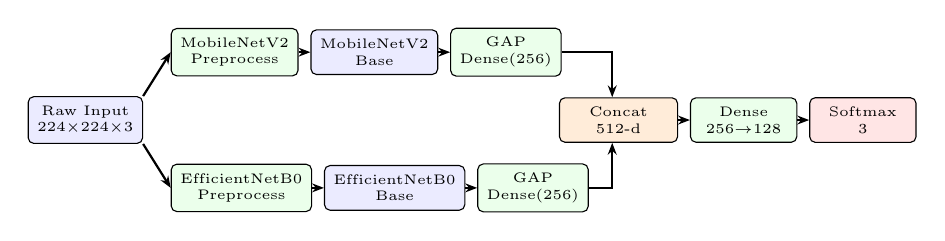
\begin{tikzpicture}[
    node distance=0.25cm and 0.35cm,
    every node/.style={font=\tiny},
    block/.style={rectangle, draw, fill=blue!8, minimum width=1.35cm, minimum height=0.45cm, align=center, rounded corners=2pt},
    process/.style={rectangle, draw, fill=green!8, minimum width=1.35cm, minimum height=0.45cm, align=center, rounded corners=2pt},
    fusion/.style={rectangle, draw, fill=orange!15, minimum width=1.5cm, minimum height=0.45cm, align=center, rounded corners=2pt},
    output/.style={rectangle, draw, fill=red!10, minimum width=1.35cm, minimum height=0.45cm, align=center, rounded corners=2pt},
    arrow/.style={-{Stealth[length=1.5mm]}, thick}
]
\node[block] (input) {Raw Input\\224$\times$224$\times$3};
\node[process, above right=0.25cm and 0.35cm of input] (mob_pre) {MobileNetV2\\Preprocess};
\node[block, right=0.15cm of mob_pre] (mob_base) {MobileNetV2\\Base};
\node[process, right=0.15cm of mob_base] (mob_gap) {GAP\\Dense(256)};
\node[process, below right=0.25cm and 0.35cm of input] (eff_pre) {EfficientNetB0\\Preprocess};
\node[block, right=0.15cm of eff_pre] (eff_base) {EfficientNetB0\\Base};
\node[process, right=0.15cm of eff_base] (eff_gap) {GAP\\Dense(256)};
\node[fusion] (concat) at ($(mob_gap.east)!0.5!(eff_gap.east)+(0.55,0)$) {Concat\\512-d};
\node[process, right=0.15cm of concat] (dense) {Dense\\256$\to$128};
\node[output, right=0.15cm of dense] (out) {Softmax\\3};
\draw[arrow] (input.north east) -- (mob_pre.west);
\draw[arrow] (input.south east) -- (eff_pre.west);
\draw[arrow] (mob_pre) -- (mob_base);
\draw[arrow] (mob_base) -- (mob_gap);
\draw[arrow] (eff_pre) -- (eff_base);
\draw[arrow] (eff_base) -- (eff_gap);
\draw[arrow] (mob_gap.east) -| ([xshift=-0.08cm]concat.north);
\draw[arrow] (eff_gap.east) -| ([xshift=-0.08cm]concat.south);
\draw[arrow] (concat) -- (dense);
\draw[arrow] (dense) -- (out);
\end{tikzpicture}
}
\caption{Dual-backbone ensemble architecture. Both backbones receive the same raw input but apply their own preprocessing before feature fusion.}
\label{fig:ensemble_arch}
\end{figure}

Both backbones receive the same eye image. MobileNetV2 rescales pixel values to $[-1, 1]$; EfficientNetB0 applies standard ImageNet normalisation. After feature extraction, global average pooling condenses each branch's output into a 256-dimensional descriptor, and the two descriptors are concatenated into a single 512-dimensional vector. A dense classification head, incorporating batch normalisation and dropout regularisation, then maps this fused representation to the three output classes.

Training proceeds in two phases. During the first 20 epochs both backbones stay frozen and only the fusion head is trained at a learning rate of $5 \times 10^{-4}$. In the second phase (up to 40 epochs), the final 30 layers of each backbone are unfrozen and fine-tuned at a much lower learning rate of $1 \times 10^{-5}$. Dynamic class weighting ($w_c = N_{\text{total}} / (K \cdot N_c)$, with $K = 3$) compensates for any sampling imbalance.

\subsection{Expert Rules Engine and Integration}
A handcrafted expert rules engine runs in parallel with the CNN classifier (Fig.~\ref{fig:expert_pipeline}) to catch physically implausible outputs.

\begin{figure}[h]
\centering
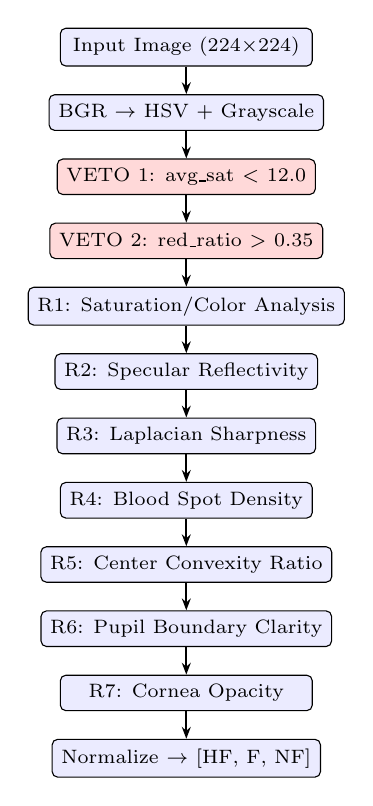
\begin{tikzpicture}[
    node distance=0.35cm,
    every node/.style={font=\scriptsize},
    block/.style={rectangle, draw, fill=blue!8, minimum width=3.2cm, minimum height=0.45cm, align=center, rounded corners=2pt},
    veto/.style={rectangle, draw, fill=red!15, minimum width=3.2cm, minimum height=0.45cm, align=center, rounded corners=2pt},
    arrow/.style={-{Stealth[length=1.5mm]}, thick}
]
\node[block] (input) {Input Image (224$\times$224)};
\node[block, below=of input] (cvt) {BGR $\to$ HSV + Grayscale};
\node[veto, below=of cvt] (v1) {VETO 1: avg\_sat $<$ 12.0};
\node[veto, below=of v1] (v2) {VETO 2: red\_ratio $>$ 0.35};
\node[block, below=of v2] (r1) {R1: Saturation/Color Analysis};
\node[block, below=of r1] (r2) {R2: Specular Reflectivity};
\node[block, below=of r2] (r3) {R3: Laplacian Sharpness};
\node[block, below=of r3] (r4) {R4: Blood Spot Density};
\node[block, below=of r4] (r5) {R5: Center Convexity Ratio};
\node[block, below=of r5] (r6) {R6: Pupil Boundary Clarity};
\node[block, below=of r6] (r7) {R7: Cornea Opacity};
\node[block, below=of r7] (norm) {Normalize $\to$ [HF, F, NF]};
\foreach \i/\j in {input/cvt, cvt/v1, v1/v2, v2/r1, r1/r2, r2/r3, r3/r4, r4/r5, r5/r6, r6/r7, r7/norm}
    \draw[arrow] (\i) -- (\j);
\end{tikzpicture}
\caption{Expert Rules Engine pipeline. Veto conditions (red) force an immediate ``Not Fresh'' label, overriding all downstream processing.}
\label{fig:expert_pipeline}
\end{figure}

Two hard-veto conditions sit at the top of the pipeline. The first fires when mean HSV saturation drops below 12.0, a hallmark of a milky, lifeless eye. The second triggers when more than 35\% of pixels fall in the red hue band ($H \in [0,10] \cup [160,180]$), indicating heavy blood contamination. If neither veto applies, the engine scores the image on seven attributes (colour saturation, specular reflectivity, Laplacian variance, blood-spot density, centre-to-periphery convexity, pupil boundary clarity, and corneal opacity) and normalises the result into a probability vector $P_{expert}$.

To limit sensitivity to bounding-box drift, Multi-View Image Test Averaging (ITA) generates four crops from each detected eye region (Table~\ref{tab:crops}). The final probability is the arithmetic mean across all four:

\begin{equation}
P_{final}(c) = \frac{1}{4} \sum_{v=1}^{4} P_{fused}^{(v)}(c), \quad c \in \{HF, F, NF\}
\end{equation}

\begin{table}[h]
\centering
\caption{Multi-View Crop Configurations}
\label{tab:crops}
\begin{tabular}{clcc}
\toprule
\textbf{Crop} & \textbf{Description} & \textbf{Padding} & \textbf{Shift} \\
\midrule
1 & Standard & 10\% & None \\
2 & Tight & 0\% & None \\
3 & Wide & 25\% & None \\
4 & Shifted & 10\% & +5\% X,Y \\
\bottomrule
\end{tabular}
\end{table}

Within each crop view the CNN ensemble probabilities $P_{CNN}$ and the expert rule probabilities $P_{expert}$ are combined through a confidence-gated fusion rule:

\begin{equation}
P_{fused} = 
\begin{cases}
P_{expert} & \text{if VETO triggered} \\
P_{CNN} & \text{if } \max(P_{CNN}) \geq 0.60 \\
0.8 \cdot P_{CNN} + 0.2 \cdot P_{expert} & \text{otherwise}
\end{cases}
\end{equation}

The CNN thus remains the primary decision-maker whenever it is confident; the expert rules step in only when the network is uncertain or when the physical evidence is conclusive.

% ═══════════════════════════════════════════════════════════════════════════════
% IV. SYSTEM DESIGN & INTEGRATION
% ═══════════════════════════════════════════════════════════════════════════════
\section{System Design \& Integration}
The system goes beyond classification by wrapping freshness assessment inside an end-to-end supply chain workflow (Fig.~\ref{fig:system_arch}). On the client side, a web application captures the fish photograph together with GPS coordinates and sends both to a REST API. The API orchestrates image enhancement, the YOLO detection cascade, multi-view crop generation, and confidence-guided fusion.

\begin{figure}[h]
\centering
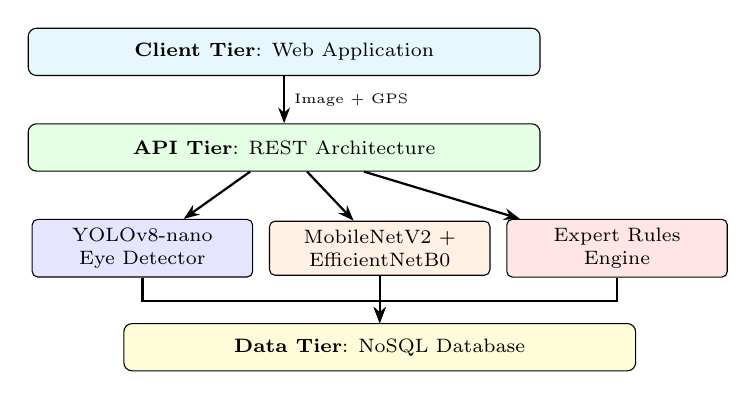
\begin{tikzpicture}[
    node distance=0.5cm and 0.4cm,
    every node/.style={font=\scriptsize},
    tier/.style={rectangle, draw, fill=#1, minimum width=6.5cm, minimum height=0.6cm, align=center, rounded corners=3pt},
    comp/.style={rectangle, draw, fill=#1, minimum width=2.8cm, minimum height=0.5cm, align=center, rounded corners=2pt},
    arrow/.style={-{Stealth[length=2mm]}, thick}
]
\node[tier=cyan!10] (client) {\textbf{Client Tier}: Web Application};
\node[tier=green!10, below=0.6cm of client] (api) {\textbf{API Tier}: REST Architecture};
\node[comp=blue!10, below=0.6cm of api, xshift=-1.8cm] (yolo) {YOLOv8-nano\\Eye Detector};
\node[comp=orange!10, right=0.2cm of yolo] (ensemble) {MobileNetV2 +\\EfficientNetB0};
\node[comp=red!10, right=0.2cm of ensemble] (expert) {Expert Rules\\Engine};
\node[tier=yellow!15, below=0.6cm of ensemble] (db) {\textbf{Data Tier}: NoSQL Database};
\draw[arrow] (client) -- node[right, font=\tiny] {Image + GPS} (api);
\draw[arrow] (api) -- (yolo);
\draw[arrow] (api) -- (ensemble);
\draw[arrow] (api) -- (expert);
\draw[arrow] (yolo.south) -- ++(0,-0.3) -| (db);
\draw[arrow] (ensemble.south) -- (db);
\draw[arrow] (expert.south) -- ++(0,-0.3) -| (db);
\end{tikzpicture}
\caption{Three-tier system architecture showing the flow from client capture through AI inference to database logging.}
\label{fig:system_arch}
\end{figure}

Once a freshness label has been assigned, the platform recommends B2B buyers whose business type matches the grade (Table~\ref{tab:routing}). Candidates are ranked by geospatial proximity using the Haversine formula \cite{ref_haversine}:

\begin{equation}
d = 2R \arcsin\sqrt{\sin^2\frac{\Delta\phi}{2} + \cos\phi_1 \cos\phi_2 \sin^2\frac{\Delta\lambda}{2}}
\end{equation}

where $R = 6{,}371$~km is Earth's mean radius, $\phi$ denotes latitude, and $\lambda$ longitude. Routing recommendations are therefore available within seconds of the photograph being taken.

\begin{table}[h]
\centering
\caption{Freshness-to-Market Routing Logic}
\label{tab:routing}
\begin{tabular}{lll}
\toprule
\textbf{Freshness} & \textbf{Target Buyers} & \textbf{Ice Rec.} \\
\midrule
Highly Fresh & Sushi bars, Hotels, Exporters & 0.5\,kg/kg \\
Fresh & Retail outlets, Supermarkets & 1\,kg/kg \\
Not Fresh & Fertiliser plants, Animal feed & Store at $-18\,^{\circ}$C \\
\bottomrule
\end{tabular}
\end{table}

% ═══════════════════════════════════════════════════════════════════════════════
% V. EXPERIMENTAL SETUP
% ═══════════════════════════════════════════════════════════════════════════════
\section{Experimental Setup}
All experiments were run in Python 3.10 with TensorFlow/Keras and OpenCV on a machine fitted with an Intel Core i5/i7 processor and 8\,GB of RAM; no GPU was used. The ensemble was trained with a batch size of 16 and categorical cross-entropy loss. Table~\ref{tab:hyperparams} lists the full set of hyperparameters. Dynamic class weights were applied to counter any class-count imbalance. Training images were augmented on the fly with random horizontal and vertical flips, 90$^{\circ}$ rotations, brightness jitter (factor 0.7 to 1.3), and random zoom crops (80 to 100\% of the original scale).

The two-phase transfer learning schedule described in Section~III was used: both ImageNet-pretrained backbones were frozen for 20~epochs while the new fusion head converged, then the last 30~layers of each backbone were unfrozen for up to 40~epochs of fine-tuning at a substantially reduced learning rate.

\begin{table}[h]
\centering
\caption{Ensemble Model Training Hyperparameters}
\label{tab:hyperparams}
\begin{tabular}{ll}
\toprule
\textbf{Parameter} & \textbf{Value} \\
\midrule
Input Size & 224 $\times$ 224 $\times$ 3 \\
Batch Size & 16 \\
Phase 1 LR & $5 \times 10^{-4}$ (Adam) \\
Phase 2 LR & $1 \times 10^{-5}$ (Adam) \\
Phase 1 Epochs & 20 (frozen backbones) \\
Phase 2 Epochs & 40 (fine-tune last 30 layers) \\
Loss Function & Categorical Cross-Entropy \\
Early Stopping Patience & 10 epochs \\
LR Reduction & Factor 0.5, patience 4 \\
Dropout (Branches) & 0.4 \\
Dropout (Fusion) & 0.3, 0.2 \\
\bottomrule
\end{tabular}
\end{table}

% ═══════════════════════════════════════════════════════════════════════════════
% VI. RESULTS AND DISCUSSION
% ═══════════════════════════════════════════════════════════════════════════════
\section{Results and Discussion}
\subsection{Ablation Study and Pipeline Performance}
Four pipeline configurations (Table~\ref{tab:ablation_configs}) were evaluated to tease apart the contribution of each component. The corresponding metrics appear in Table~\ref{tab:ablation_results}.

\begin{table}[h]
\centering
\caption{Ablation Study Configuration Matrix}
\label{tab:ablation_configs}
\begin{tabular}{ccccc}
\toprule
\textbf{Config} & \textbf{CNN} & \textbf{Multi-View} & \textbf{Expert} & \textbf{Fusion} \\
\midrule
A & Ensemble & \texttimes & \texttimes & CNN only \\
B & Ensemble & \checkmark & \texttimes & 4-crop avg \\
C & Ensemble & \texttimes & \checkmark & 80/20 + Veto \\
D & Ensemble & \checkmark & \checkmark & Full hybrid \\
\bottomrule
\end{tabular}
\end{table}

\begin{table}[h]
\centering
\caption{Ablation Study: Configuration Comparison}
\label{tab:ablation_results}
\begin{tabular}{lccccc}
\toprule
\textbf{Config} & \textbf{Acc.} & \textbf{M-Prec} & \textbf{M-Rec} & \textbf{M-F1} & \textbf{M-AUC} \\
\midrule
A: CNN Only & 69.34\% & 70.88\% & 69.34\% & 69.34\% & 0.8695 \\
B: CNN+MV & 69.34\% & 70.88\% & 69.34\% & 69.34\% & 0.8695 \\
C: CNN+ER & 68.32\% & 69.74\% & 68.32\% & 68.20\% & 0.8576 \\
D: Full & 68.32\% & 69.74\% & 68.32\% & 68.20\% & 0.8576 \\
\bottomrule
\end{tabular}
\end{table}

The bare dual-backbone CNN (Config~A) reached 69.34\% validation accuracy (Table~\ref{tab:config_a_detail}). Adding Multi-View ITA (Config~B) left these numbers unchanged, which is expected: the validation images are already cleanly cropped eye patches, so generating alternative crops does not introduce new information. In a live deployment, where the detector's bounding box may wobble by several pixels, Multi-View averaging is expected to provide a measurable benefit.

\begin{table}[h]
\centering
\caption{Configuration A: Per-Class Detailed Metrics}
\label{tab:config_a_detail}
\begin{tabular}{lccccc}
\toprule
\textbf{Class} & \textbf{Prec.} & \textbf{Recall} & \textbf{F1} & \textbf{AUC} & \textbf{Sup.} \\
\midrule
Fresh & 58.26\% & 74.05\% & 65.21\% & 0.8212 & 262 \\
Highly Fresh & 79.38\% & 77.86\% & 78.61\% & 0.9162 & 262 \\
Not Fresh & 75.00\% & 56.11\% & 64.19\% & 0.8712 & 262 \\
\midrule
\textbf{Macro Avg} & \textbf{70.88\%} & \textbf{69.34\%} & \textbf{69.34\%} & \textbf{0.8695} & \textbf{786} \\
\bottomrule
\end{tabular}
\end{table}

Switching on the expert rules engine (Config~C) drops accuracy to 68.32\% (Table~\ref{tab:config_d_detail}). Config~D, which combines expert rules with Multi-View ITA, records the same 68.32\% for the same reason that B matched A: the pre-cropped validation images give Multi-View averaging nothing extra to work with. The 1.02-percentage-point decrease caused by the rules engine is a deliberate trade-off. On a handful of visually ambiguous samples the fixed rules overwrite a correct CNN prediction, but they guarantee that no clearly milky or blood-contaminated eye is ever labelled ``Highly Fresh,'' which would be unacceptable in a food-safety context.

\begin{table}[h]
\centering
\caption{Configuration D (Production): Per-Class Detailed Metrics}
\label{tab:config_d_detail}
\begin{tabular}{lccccc}
\toprule
\textbf{Class} & \textbf{Prec.} & \textbf{Recall} & \textbf{F1} & \textbf{AUC} & \textbf{Sup.} \\
\midrule
Fresh & 58.08\% & 74.05\% & 65.10\% & 0.8153 & 262 \\
Highly Fresh & 77.69\% & 77.10\% & 77.39\% & 0.8975 & 262 \\
Not Fresh & 73.44\% & 53.82\% & 62.11\% & 0.8601 & 262 \\
\midrule
\textbf{Macro Avg} & \textbf{69.74\%} & \textbf{68.32\%} & \textbf{68.20\%} & \textbf{0.8576} & \textbf{786} \\
\bottomrule
\end{tabular}
\end{table}

\subsection{Error Analysis and Confusion Matrices}
Two error patterns stand out in the confusion matrices (Table~\ref{tab:confusion}). The most frequent mistake is labelling a ``Not Fresh'' sample as ``Fresh'' (94 to 96 instances): fish in the early stages of spoilage can still look reasonably clear-eyed, making the boundary genuinely hard to draw. The second pattern is a ``Fresh'' sample being called ``Highly Fresh'' (32 to 33 instances), usually because wet-surface glare mimics the specular highlights typical of a very fresh eye.

\begin{table}[h]
\centering
\caption{Confusion Matrices (Rows: Actual, Columns: Predicted)}
\label{tab:confusion}
\begin{tabular}{c|ccc|c|ccc}
\toprule
\multicolumn{4}{c|}{\textbf{Config A (CNN Only)}} & \multicolumn{4}{c}{\textbf{Config D (Full Hybrid)}} \\
\midrule
& F & HF & NF & & F & HF & NF \\
\midrule
F & \textbf{194} & 32 & 36 & F & \textbf{194} & 33 & 35 \\
HF & 45 & \textbf{204} & 13 & HF & 44 & \textbf{202} & 16 \\
NF & 94 & 21 & \textbf{147} & NF & 96 & 25 & \textbf{141} \\
\bottomrule
\end{tabular}
\end{table}

\subsection{Parameter Sweep of Decision-Level Fusion Weights}
A natural question is whether simply blending the probability outputs of the two backbones at decision level could match the feature-level fusion used in the ensemble. To find out, a parameter sweep was run:

\begin{equation}
P_{\text{final}} = w_{\text{mob}} \cdot P_{\text{MobileNet}} + w_{\text{eff}} \cdot P_{\text{EfficientNet}}
\end{equation}

Table~\ref{tab:weight_sweep} shows the results. EfficientNetB0 alone (63.87\%) outperforms MobileNetV2 alone (57.76\%), and the best linear blend (40/60 split) tops out at 68.32\%. That is still a full percentage point below the 69.34\% achieved by concatenating feature vectors and letting a shared dense head learn non-linear combinations, which confirms that feature-level fusion captures complementary information that simple probability averaging cannot.

\begin{table}[h]
\centering
\caption{Accuracy Across Prediction Probability Weights}
\label{tab:weight_sweep}
\begin{tabular}{ccc}
\toprule
\textbf{Weight (MobileNet)} & \textbf{Weight (EfficientNet)} & \textbf{Accuracy} \\
\midrule
1.00 (MobileNet Only) & 0.00 & 57.76\% \\
0.90 & 0.10 & 59.16\% \\
0.80 & 0.20 & 61.70\% \\
0.70 & 0.30 & 64.50\% \\
0.60 & 0.40 & 66.41\% \\
0.50 & 0.50 & 67.18\% \\
0.40 & 0.60 (Best Blend) & 68.32\% \\
0.30 & 0.70 & 66.79\% \\
0.20 & 0.80 & 66.67\% \\
0.10 & 0.90 & 65.27\% \\
0.00 & 1.00 (EfficientNet Only) & 63.87\% \\
\midrule
\multicolumn{2}{c}{\textbf{Native Feature Concatenation (Ours)}} & \textbf{69.34\%} \\
\bottomrule
\end{tabular}
\end{table}

\subsection{Comparison with Existing Literature}
Table~\ref{tab:comparison_new} places the proposed framework alongside representative alternatives. Several academic studies report near-perfect accuracy on curated laboratory datasets \cite{ref19}, but such numbers are difficult to reproduce once image quality varies, as it inevitably does at an actual market stall. Instrumental techniques built on hyperspectral imaging or chemical assays deliver molecular-level reliability \cite{ref3, ref18}, at the cost of specialised hardware or destructive sample preparation. The present system deliberately sacrifices top-end laboratory accuracy in exchange for field robustness and actionable supply-chain output from a commodity smartphone camera.

\begin{table}[h]
\centering
\caption{Comparison with Existing Freshness Detection Systems}
\label{tab:comparison_new}
\begin{tabular}{>{\raggedright\arraybackslash}p{1.8cm} >{\raggedright\arraybackslash}p{2.5cm} >{\raggedright\arraybackslash}p{1.2cm} >{\raggedright\arraybackslash}p{2cm}}
\toprule
\textbf{System} & \textbf{Approach Type} & \textbf{Reported Metric} & \textbf{Key Trade-Off} \\
\midrule
FishSense\footnotemark[1] & Open-source, rule-based only & N/A & Lightweight but brittle; no supply chain output. \\
\rowcolor{gray!10}
Yildiz \textit{et al.} \cite{ref19} & Deep learning + SVM/RF & up to 100\% & Curated lab data; no field fallbacks. \\
Banwari\footnotemark[2] & Traditional CV (colour tracking) & 96.67\% & Collapses under wet glare and lighting artefacts. \\
\rowcolor{gray!10}
Instrumental \cite{ref3,ref18} & Hyperspectral / NIR / TVB-N & Molecular accuracy & Destructive or \$10k+ hardware. \\
\textbf{Proposed} & \textbf{Hybrid CNN + Expert Rules} & \textbf{69.34\%} (Field) & Trades lab accuracy for field actionability. \\
\bottomrule
\end{tabular}
\end{table}

\footnotetext[1]{FishSense, open-source repository: \url{https://github.com/FishSense}}
\footnotetext[2]{D. Banwari, ``Fish freshness detection using color tracking,'' unpublished project report, 2020.}

% ═══════════════════════════════════════════════════════════════════════════════
% VII. CONCLUSION
% ═══════════════════════════════════════════════════════════════════════════════
\section{Conclusion}
This paper has described a hybrid framework for grading fish freshness from smartphone photographs of the eye. By pairing a combined MobileNetV2 and EfficientNetB0 ensemble with a deterministic expert rules engine and Multi-View Image Test Averaging, the system reaches 69.34\% accuracy and a macro ROC-AUC of 0.8695 on field-captured images, without needing any specialised equipment. The ablation study shows that most of the performance gain comes from the dual-backbone fusion, while the expert rules engine contributes a safety layer that prevents physically absurd misclassifications at the expense of a small accuracy dip. Plugging the classifier into a geodistance-based B2B marketplace closes the loop between quality assessment and commercial decision-making, allowing routing suggestions to appear within seconds of the photograph being taken.

% ═══════════════════════════════════════════════════════════════════════════════
% VIII. LIMITATIONS AND FUTURE WORK
% ═══════════════════════════════════════════════════════════════════════════════
\section{Limitations and Future Work}
The ``Fresh'' class remains the hardest to get right, because wet-glare artefacts on a moderately fresh eye can look much like the specular highlights of a truly fresh one. Running four crop views per prediction also adds computational overhead compared with a single-crop pipeline. Going forward, collecting more images across a wider range of species and lighting conditions should sharpen the class boundaries. On the architectural side, Vision Transformers (ViT) could serve as a third ensemble backbone, and channel-attention modules such as CBAM may help the network focus on discriminative eye features while down-weighting glare. Porting the CNN to TensorFlow Lite would also open the door to on-device inference in remote coastal areas where connectivity is unreliable.

% ═══════════════════════════════════════════════════════════════════════════════
% REFERENCES
% ═══════════════════════════════════════════════════════════════════════════════
\balance
\begin{thebibliography}{00}
\bibitem{ref1}
L. Wu, H. Pu, and D.-W. Sun, ``Novel techniques for evaluating freshness quality attributes of fish: A review of recent developments,'' \textit{Trends Food Sci. Technol.}, vol. 83, pp. 259--273, Jan. 2019, doi: 10.1016/j.tifs.2018.12.002.

\bibitem{ref20}
S. Ismail, D. W. Nadim Reyes, and A. Dawoud, ``Toward an intelligent blockchain IoT-enabled fish supply chain: A review and conceptual framework,'' \textit{Sensors}, vol. 23, no. 11, art. no. 5136, May 2023, doi: 10.3390/s23115136.

\bibitem{ref6}
A. Hassoun and R. Karoui, ``Quality evaluation of fish and other seafood by traditional and nondestructive instrumental methods: Advantages and limitations,'' \textit{Crit. Rev. Food Sci. Nutr.}, vol. 57, no. 9, pp. 1976--1998, Jun. 2017, doi: 10.1080/10408398.2015.1047926.

\bibitem{ref18}
J. H. T. Luong, K. B. Male, C. Masson, and A. L. Nguyen, ``Hypoxanthine ratio determination in fish extract using capillary electrophoresis and immobilized enzymes,'' \textit{J. Food Sci.}, vol. 57, no. 1, pp. 77--81, Jan. 1992, doi: 10.1111/j.1365-2621.1992.tb05429.x.

\bibitem{ref3}
J. Qin, M. S. Kim, K. Chao, D. E. Chan, S. R. Delwiche, and B.-K. Cho, ``Detection of fish fillet substitution and mislabeling using multimode hyperspectral imaging techniques,'' \textit{Food Control}, vol. 114, art. no. 107234, Aug. 2020, doi: 10.1016/j.foodcont.2020.107234.

\bibitem{ref13}
C. McVey, C. T. Elliott, A. Cannavan, S. D. Kelly, A. Petchkongkaew, and S. A. Haughey, ``A rapid food chain approach for authenticity screening: Using two handheld near-infrared spectroscopy devices to distinguish between key oregano species,'' \textit{Talanta}, vol. 222, art. no. 121533, Jan. 2021, doi: 10.1016/j.talanta.2020.121533.

\bibitem{ref19}
M. B. Yildiz, E. T. Yasin, and M. Koklu, ``Fisheye freshness detection using common deep learning algorithms and machine learning methods with a developed mobile application,'' \textit{Eur. Food Res. Technol.}, vol. 250, no. 7, pp. 1919--1932, Jul. 2024, doi: 10.1007/s00217-024-04493-0.

\bibitem{ref4}
J. Chauvin, R. Duran, S. Tavakolian, N. Alizadeh Sabet, and R. Ghaffari, ``Simulated annealing-based hyperspectral data optimization for fish species classification: Can the number of measured wavelengths be reduced?,'' \textit{Appl. Sci.}, vol. 11, no. 22, art. no. 10628, Nov. 2021, doi: 10.3390/app112210628.

\bibitem{ref5}
J.-H. Cheng, D.-W. Sun, H. Pu, and Z. Zhu, ``Development of hyperspectral imaging coupled with chemometric analysis to monitor K value for evaluation of chemical spoilage in fish fillets,'' \textit{Food Chem.}, vol. 185, pp. 245--253, Oct. 2015, doi: 10.1016/j.foodchem.2015.03.111.

\bibitem{ref7}
A. Hassoun, A. Sahar, L. Lakhal, and A. A{\"i}t-Kaddour, ``Emerging techniques for differentiation of fresh and frozen-thawed seafoods: Highlighting the potential of spectroscopic techniques,'' \textit{Molecules}, vol. 25, no. 19, art. no. 4472, Sep. 2020, doi: 10.3390/molecules25194472.

\bibitem{ref8}
{\'E}. Dufour, J. P. Frencia, and E. Kane, ``Development of a rapid method based on front-face fluorescence spectroscopy for the monitoring of fish freshness,'' \textit{Food Res. Int.}, vol. 36, no. 5, pp. 415--423, Jun. 2003, doi: 10.1016/S0963-9969(02)00174-6.

\bibitem{ref9}
G. ElMasry, K. Nakazawa, S. Okazawa, and S. Nakauchi, ``Freshness estimation of intact frozen fish using fluorescence spectroscopy and chemometrics of excitation-emission matrix,'' \textit{Talanta}, vol. 143, pp. 145--156, Oct. 2015, doi: 10.1016/j.talanta.2015.05.031.

\bibitem{ref10}
R. Karoui, A. Hassoun, and P. Ethuin, ``Front face fluorescence spectroscopy enables rapid differentiation of fresh and frozen-thawed sea bass (\textit{Dicentrarchus labrax}) fillets,'' \textit{J. Food Eng.}, vol. 202, pp. 89--98, Jun. 2017, doi: 10.1016/j.jfoodeng.2017.01.018.

\bibitem{ref11}
K. A. Omwange \textit{et al.}, ``Japanese dace (\textit{Tribolodon hakonensis}) fish freshness estimation from eyes using front-face fluorescence spectroscopy and hyperspectral imaging,'' \textit{Spectrochim. Acta A, Mol. Biomol. Spectrosc.}, vol. 276, art. no. 121209, Jul. 2022, doi: 10.1016/j.saa.2022.121209.

\bibitem{ref12}
S. Khoshnoudi-Nia and M. Moosavi-Nasab, ``Prediction of various freshness indicators in fish fillets by one multispectral imaging system,'' \textit{Sci. Rep.}, vol. 9, art. no. 14704, Oct. 2019, doi: 10.1038/s41598-019-51264-z.

\bibitem{ref14}
C. McVey \textit{et al.}, ``Assessment of the analytical performance of three near-infrared spectroscopy instruments (benchtop, handheld and portable) through the investigation of coriander seed authenticity,'' \textit{Foods}, vol. 10, no. 5, art. no. 956, Apr. 2021, doi: 10.3390/foods10050956.

\bibitem{ref2}
J. M{\"u}ller-Maatsch and S. M. van Ruth, ``Handheld devices for food authentication and their applications: A review,'' \textit{Foods}, vol. 10, no. 12, art. no. 2901, Nov. 2021, doi: 10.3390/foods10122901.

\bibitem{ref15}
R. Wehrens and L. M. C. Buydens, ``Self- and super-organizing maps in R: The kohonen package,'' \textit{J. Stat. Softw.}, vol. 21, no. 5, pp. 1--19, Oct. 2007, doi: 10.18637/jss.v021.i05.

\bibitem{ref16}
J. R. Beattie and F. W. L. Esmonde-White, ``Exploration of principal component analysis: Deriving principal component analysis visually using spectra,'' \textit{Appl. Spectrosc.}, vol. 75, no. 4, pp. 361--375, Apr. 2021, doi: 10.1177/0003702820987847.

\bibitem{ref17}
H. F. Kaiser, ``The application of electronic computers to factor analysis,'' \textit{Educ. Psychol. Meas.}, vol. 20, no. 1, pp. 141--151, Apr. 1960, doi: 10.1177/001316446002000116.

\bibitem{ref23}
G. Jocher, A. Chaurasia, and J. Qiu, ``YOLO by Ultralytics (Version 8.0.0),'' GitHub repository, 2023. [Online]. Available: https://github.com/ultralytics/ultralytics

\bibitem{ref21}
M. Sandler, A. Howard, M. Zhu, A. Zhmoginov, and L.-C. Chen, ``MobileNetV2: Inverted residuals and linear bottlenecks,'' in \textit{Proc. IEEE/CVF Conf. Comput. Vis. Pattern Recognit. (CVPR)}, Salt Lake City, UT, USA, Jun. 2018, pp. 4510--4520, doi: 10.1109/CVPR.2018.00474.

\bibitem{ref22}
M. Tan and Q. V. Le, ``EfficientNet: Rethinking model scaling for convolutional neural networks,'' in \textit{Proc. 36th Int. Conf. Mach. Learn. (ICML)}, Long Beach, CA, USA, vol. 97, Jun. 2019, pp. 6105--6114.

\bibitem{ref_haversine}
R. W. Sinnott, ``Virtues of the Haversine,'' \textit{Sky Telesc.}, vol. 68, no. 2, p. 159, Aug. 1984.

\bibitem{ref_roc}
T. Fawcett, ``An introduction to ROC analysis,'' \textit{Pattern Recognit. Lett.}, vol. 27, no. 8, pp. 861--874, Jun. 2006, doi: 10.1016/j.patrec.2005.10.010.
\end{thebibliography}
\end{document}
